\documentclass[10pt,a4paper]{article}
\usepackage[utf8]{inputenc}
\usepackage{amsmath}
\usepackage{amsfonts}
\usepackage{amssymb}
\usepackage{graphicx}
\author{FILIP STENBECK	930702-4530 \\ ALEXANDER RAMM 931005-8418}
\date{Febuary 2016}
\title{Homework 2}
\begin{document}
\maketitle
\clearpage
\section*{Part 1:}
\subsection*{Rate Monotonic scheduling}
\subsubsection*{1}
Rate monotonic scheduling is a scheduling algorithm with fixed priorities. The highest priority is designated to the task with lowest period $T_i$. 
\subsubsection*{2}
The rate monotonic algorithm is schedulable if the Utilization factor ($U$) is less than $ln(2)$.
\begin{equation*}
U=\sum_{
   i=1
  }^{3}
 \frac{C_i}{T_i}<ln(2)
\end{equation*}
for these tasks with $C_1=C_2=C_3=6 ms$ the utilization factor is $0.6783$ which is less than $ln(2)$ thus scheduable.
\begin{figure}[!h]
  \centering
    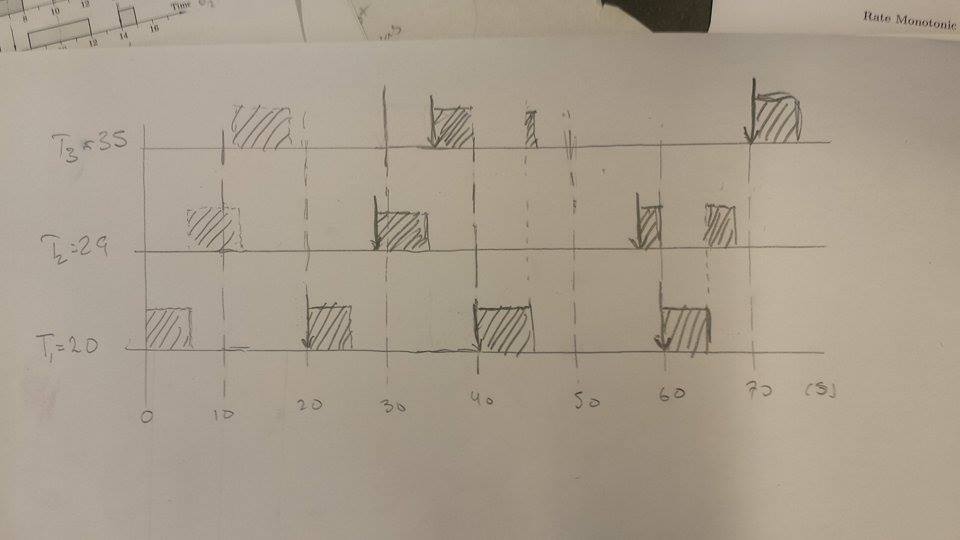
\includegraphics[width=0.8\textwidth]{egen.jpg}
      \caption{The schedual for the three pendulums, for the first 70 ms.}
\end{figure}
\subsubsection*{3}
\begin{figure}[!ht]
  \centering
    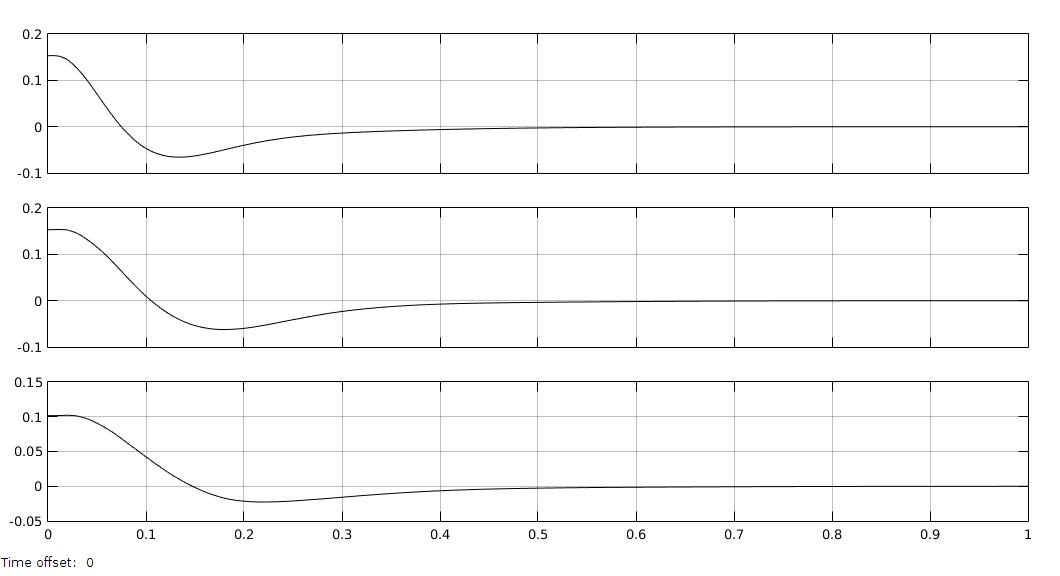
\includegraphics[width=1\textwidth]{6ms.jpg}
      \caption{All three pendulums seems to be stable at execution time 6 ms.}
\end{figure}
The three pendulums have similar performances but we can see that there is no delay in the pendulum with highest priority (top plot) whilst the two other pendulums have a 6, 12 ms delay since they have lower priority. Due to that the system is scheduable we note that all the task are performed though with a maximum delay of 35 ms for the pendulum with lowest priority. 
\newpage
\subsubsection*{4}
\begin{figure}[!h]
  \centering
    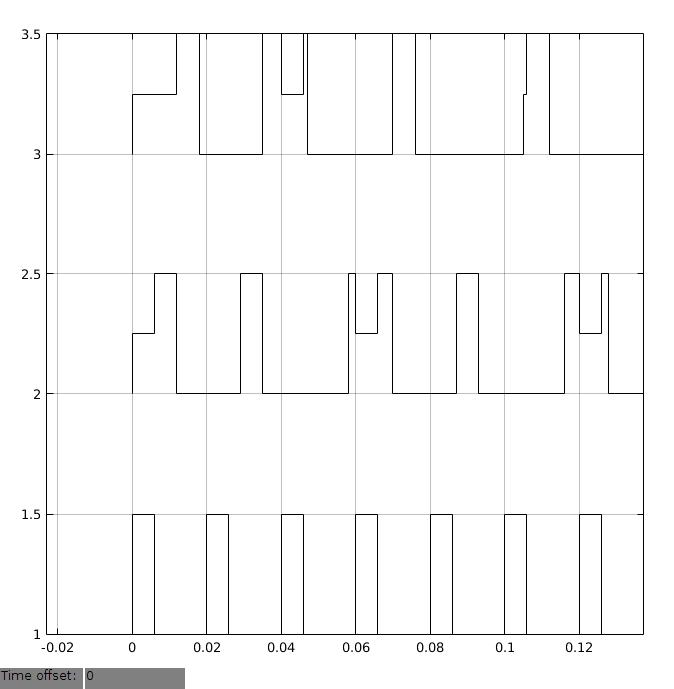
\includegraphics[width=0.8\textwidth]{schedual6ms.jpg}
      \caption{The schedual for the three pendulums, highest priority is the bottom plot, lowest priority is the top plot. As we can see the analytic plot does seem to map to the schedule plot from simulink over the first 80 ms.}
\end{figure}
\subsubsection*{5}
For the tasks with $C_1=C_2=C_3=10 ms$ the utilization factor is $1.13$ which is higher than $ln(2)$ thus not scheduable. Note: Only the two tasks with the highest priority results in a utilization factor of $0.84$ which is still not scheduable, though this does not necessarily mean task 2 should be unstable as seen in figure \ref{1} but only that some data loss will happen.
\begin{figure}[!h]\label{1}
  \centering
    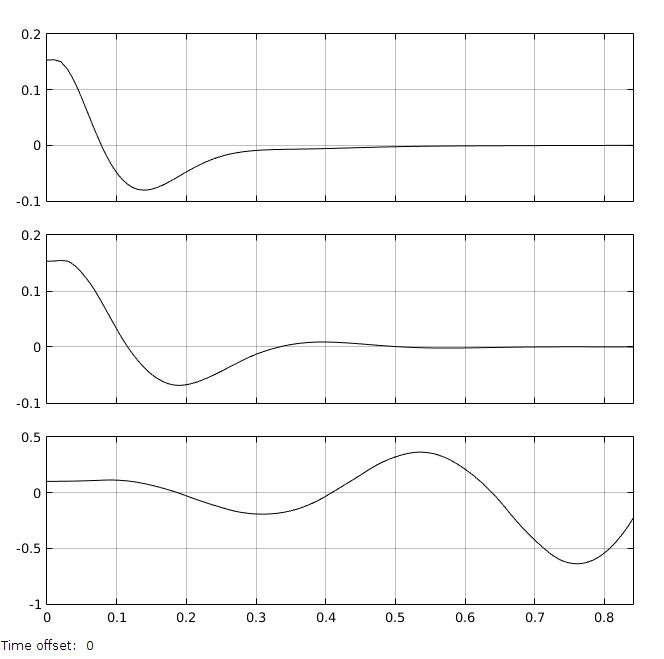
\includegraphics[width=0.7\textwidth]{10ms.jpg}
      \caption{The pendulum with the lowest priority is now unstable at execution time 10 ms.}
\end{figure}
\newpage
\subsection*{Earliest deadline first}
\subsubsection*{1}
Earliest deadline first (EDF) is a dynamic scheduling algorithm. It calculates the closest deadline in absolute time and sets the priority according to that. This optimizes the computer time to the task in most need of it, thus making systems stable as long as the utilization factor is lower than 1. Since the algorithm is dynamic the computer need to continuously calculate the priorities of the tasks which does take some computation power and is slightly more complex than the predefined priorities from the rate monotonic algorithm.
\subsubsection*{2}  
The utilization factor is still $0.6783<1$ thus scheduable with this method.
\begin{figure}[!h]
  \centering
    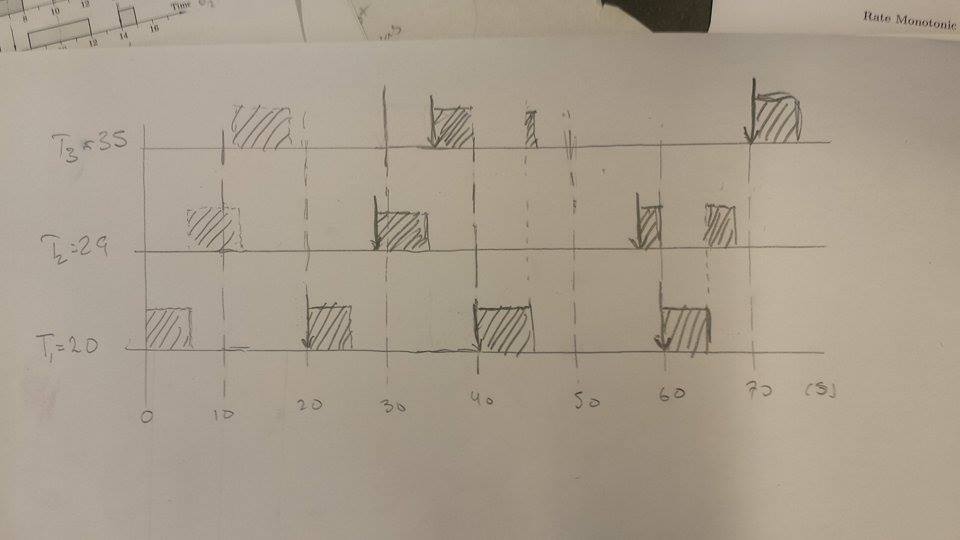
\includegraphics[width=0.8\textwidth]{egen.jpg}
      \caption{The schedual for the three pendulums, for the first 70 ms. This is just the same as the rate monotonic algorithm for this interval.}
\end{figure}
\subsubsection*{3}
\begin{figure}[!ht]
  \centering
    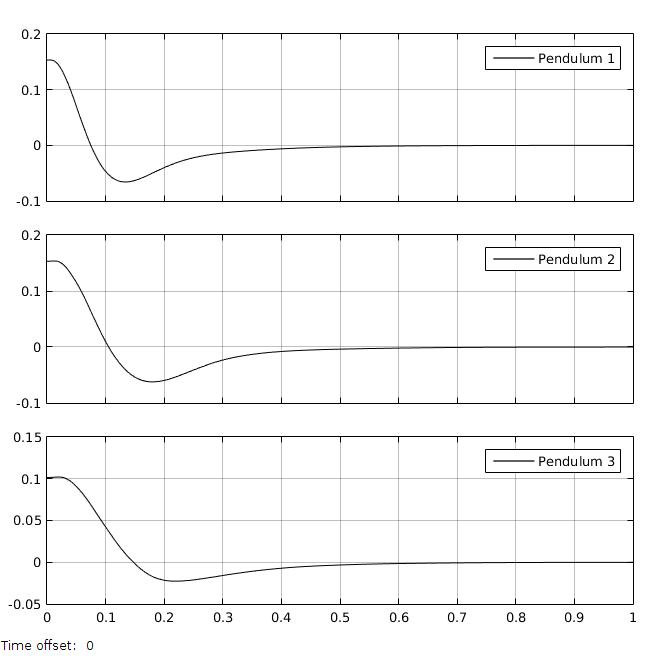
\includegraphics[width=1\textwidth]{6msedf.jpg}
      \caption{All three pendulums seems to be stable at execution time 6 ms with the EDF algorithm.}
\end{figure}
Just like for the Rate monotonic algorithm for these execution times the three pendulums are stable. The shortest pendulum seem to have a little bit quicker response time. This is due to that it will be executed first at time $0(s)$. 
\subsubsection*{4}
\begin{figure}[!h]
  \centering
    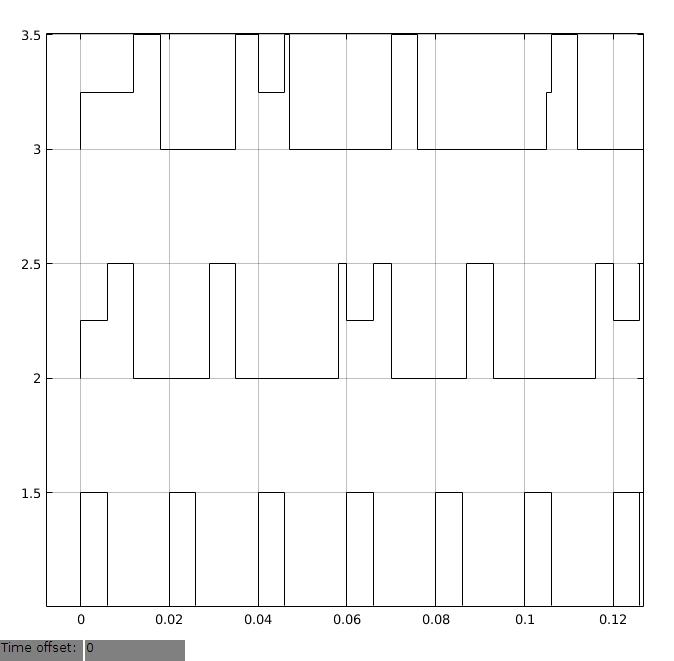
\includegraphics[width=0.8\textwidth]{schedual6msedf.jpg}
      \caption{The schedual for the three pendulums,longest pendulum in the bottom plot, shortest in the top plot. As we can see the analytic plot maps to the schedule plot from simulink over the first 80 ms.}
\end{figure}
\subsubsection*{5}
The utilization factor is still $1.13>1$ thus not scheduable with this method.
\begin{figure}[!h]
  \centering
    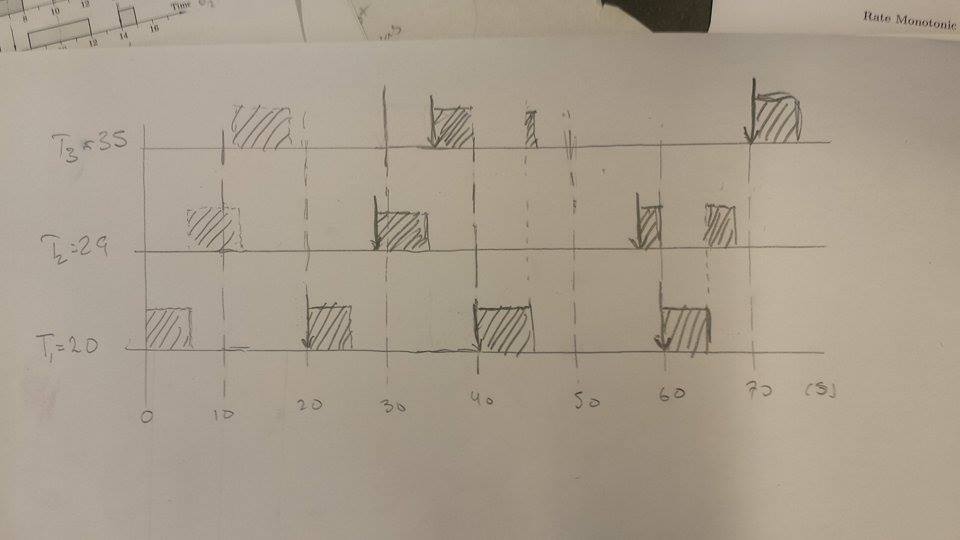
\includegraphics[width=0.8\textwidth]{egen.jpg}
      \caption{The schedual for the three pendulums, for the first 70 ms.}
\end{figure}
\begin{figure}[!h]
  \centering
    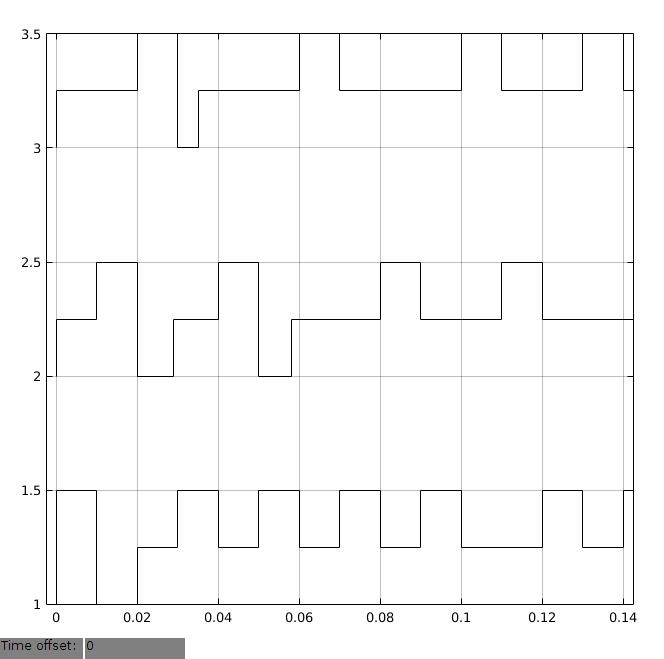
\includegraphics[width=0.8\textwidth]{schedual10msedf.jpg}
      \caption{The schedual for the three pendulums, at $C_i=10$ ms. We see that sometimes the first pendulum does not have the highest priority unlike the RM algorithm}
\end{figure}
\begin{figure}[!h]
  \centering
    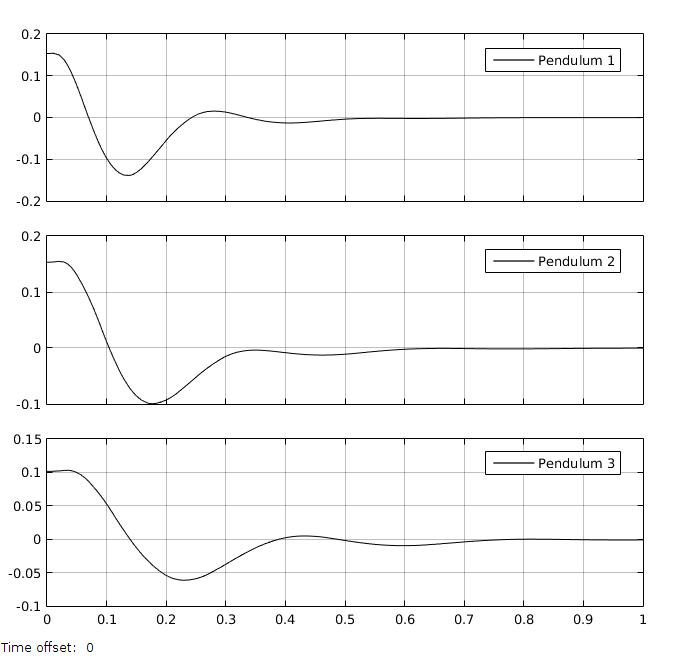
\includegraphics[width=0.8\textwidth]{10msedf.jpg}
      \caption{The step response for the three pendulums with execution time 10 ms. We see that all three systems are stable unlike the RM algorithm, though we see that pendulum 1 has far worse performance.}
\end{figure}

\newpage
\section*{Part 2:}
\subsection*{1. " Calculate analytically the closed-loop equations of the system."}
The following network control system is given. 
\begin{equation}
\dot{x}=Ax+Bu
\end{equation}\\ Where the matrices $A$, $B$ are set to be $0$, $I$ since the system is a simple integrator. The input $u$ is set to be. \\
\begin{equation*}
u=-Kx
\end{equation*}\\
In the network two delays are introduced. One before and one after the controller. This results in that the input of the system is delayed $\tau_{sc}+\tau_{ea}$ seconds. Since $\tau_{sc}+\tau_{ea}<h$ the input signal can be written.\\
\begin{equation}\label{knep1}
u=
\begin{cases}
u_0=-Kx(kh-h)&kh<t<kh+\tau_{sc}+\tau_{ea}\\
u_1=-Kx(kh)&kh+\tau_{sc}+\tau_{ea}<t<kh+h
\end{cases}
\end{equation}
With this we can formulate the closed loop equation.
\begin{equation*}
x(kh+h)=\mathrm{e}^{Ah}+\int_{kh}^{kh+h} \mathrm{e}^{AS}\,\mathrm{d}S Bu
\end{equation*}
\begin{equation}\label{knep2}
=\mathrm{e}^{Ah}x(kh)+\int_{kh}^{kh+\tau_{sc}+\tau_{ea}} \mathrm{e}^{AS}\,\mathrm{d}S Bu_0+\int_{kh+\tau_{sc}+\tau_{ea}}^{kh+h} \mathrm{e}^{AS}\,\mathrm{d}S Bu_1
\end{equation}
Setting the time delay $\tau=\tau_{sc}+\tau_{ea}$ and combining the equations \ref{knep1} with \ref{knep2} we result in the following closed loop equation.
\begin{equation*}
x(kh+h)=\begin{bmatrix}
1+K(\tau-h)&0\\
0&-K\tau
\end{bmatrix}
\begin{bmatrix}
x(kh)\\
x(kh-1)
\end{bmatrix}
\end{equation*}
\subsection*{2}
Since the continuous plant is a simple integrator $G(s)=\frac{1}{s}$ we get that the zero-order hold of the continuous plant will have the following pulse-transfer function.
\begin{equation*}
H(z)=\frac{h}{z-1}
\end{equation*}
With the controller as $C(z)=-K$ we will have a stable system if.
\begin{equation*}
|\frac{G(z)C(z)}{1+G(z)C(z)}|<\frac{1}{\tau z},	z\in R
\end{equation*}
This can be written as.
\begin{equation*}
hK(1-z\tau)<z-1,	z\in R
\end{equation*}





\end{document}